\section{Auswertung}
\label{sec:Auswertung}

Zur Untersuchung der Charakteristik des Geiger-Müller-Zählrohres werden die Daten aus \autoref{tab:charak} betrachtet.

\begin{table}[!htp]
\centering
\caption{Daten zur Bestimmung der Charakteristik des Geiger-Müller-Zählrohres.}
\label{tab:charak}
\begin{tabular}{S[table-format=3.0] S[table-format=5.0] S[table-format=3.0] S[table-format=2.1] c}
\toprule
{$U$ / V} & {$N$} & {$\Delta N$} & {$\frac{N}{t}$ / $\frac{1}{\symup{s}}$} & {$I$ / µA} \\
\midrule
320 & 11073 & 105 & 73.8 & - \\
340 & 11100 & 105 & 74.0 & - \\
360 & 11095 & 105 & 74.0 & - \\
380 & 11045 & 105 & 73.6 & 0.2 \\
400 & 11231 & 106 & 74.9 & - \\
420 & 11290 & 106 & 75.3 & - \\
440 & 11147 & 106 & 74.3 & - \\
460 & 11236 & 106 & 74.9 & - \\
480 & 11170 & 106 & 74.5 & - \\
500 & 11241 & 106 & 75.0 & - \\
520 & 11174 & 106 & 74.5 & 0.4 \\
540 & 11207 & 106 & 74.7 & - \\
560 & 11387 & 107 & 75.9 & - \\
580 & 11253 & 106 & 75.0 & - \\
600 & 11438 & 107 & 76.3 & - \\
620 & 11207 & 106 & 74.7 & - \\
640 & 11319 & 106 & 75.5 & - \\
660 & 11197 & 106 & 74.6 & - \\
680 & 11444 & 107 & 76.3 & 0.6 \\
\bottomrule
\end{tabular}
\end{table}

Zunächst wird in einem Plot $\frac{N}{t}$ gegen $U$ aufgetragen. Dabei ist $t = 150 \, \symup{s}$.
Anschließend wird durch den linearen Teil, welcher hier der gesamte Bereich ist, eine Ausgleichsgerade der Form

\begin{equation}
    \frac{N}{t} = a U + b
\end{equation}

gelegt.

\begin{figure}
  \centering
  \includegraphics[width=0.95\textwidth]{build/plot_charak.pdf}
  \caption{Plot und Fit von $\frac{N}{t}$ gegen $U$ zur Bestimmung der Charakteristik des Zählrohres.}
  \label{fig:charak}
\end{figure}

Der somit entstehende Plot ist in \autoref{fig:charak} zu sehen.
Mittels des Python 3.7.0 Paketes Curve Fit ergeben sich zu Koeffizienten zu

\begin{align*}
    a = (4,789 \pm 0,001) \cdot 10^{-3} \, \frac{1}{\symup{Vs}}\\
    b = (72,3 \pm 0,4) \, \frac{1}{\symup{s}}.
\end{align*}

Zur Bestimmung der Steigung des Plateaus wird die Formel

\begin{equation}
    s = \frac{\dot{n}_+ - \dot{n}_-}{\dot{n}_m}
\end{equation}

genutzt, wobei $\dot{n}_i = a \cdot U_i + b$ die Zählraten zu den jeweiligen Spannung sind.
Es wird $\dot{n}_m$ bei $U_m = 500$ V und $\dot{n}_\pm$ an jeweils $U_\pm = (500 \pm 50)$ V, um so eine Normierung auf $\frac{\%}{100\symup{V}}$ zu erhalten.

Damit ergibt sich für die Steigung

\begin{center}
    $s = (0,641 \pm 0,003)$ $\frac{\%}{100\symup{V}}$,
\end{center}

wobei sich der Fehler nach Gauß über

\begin{equation}
    \Delta s^2 = \bigg( \dfrac{b\left(2 U_m - U_- -U_+ \right)}{\left(a U_m + b \right)^2} \bigg)^2 \cdot \Delta a^2 + \bigg( \dfrac{a\left(2U_m - U_- - U_+ \right)}{\left(a U_m + b \right)^2} \bigg)^2 \cdot \Delta b^2
\end{equation}

berechnet.

\begin{table}[!htp]
\centering
\caption{Daten der Messung mit zwei Proben zur Bestimmung der Totzeit des Geiger-Müller-Zählrohres.}
\label{tab:tot}
\begin{tabular}{c S[table-format=5.0] @{${}\pm{}$} S[table-format=3.0] S[table-format=3.0]}
\toprule
{Probe} & \multicolumn{2}{c}{$N$} & {$\frac{N}{t}$ / $\frac{1}{\symup{s}}$} \\
\midrule
$1$ & 12914 & 114 & 215 \\
$2$ & 15790 & 126 & 263 \\
${1+2}$ & 27965 & 167 & 466 \\
\bottomrule
\end{tabular}
\end{table}

%TODO: Gleichung
Zur Bestimmung der Totzeit des Rohres werden die Daten aus \autoref{tab:tot} verwendet.
Dabei beträgt die Messdauer $t = 60$ s.
Gemäß GLEICHUNG wird die Totzeit als

\begin{center}
    $T_\text{Doppel} = (1,1 \pm 0,3) \cdot 10^{-4}$ s.
\end{center}

bestimmt. Dabei ist der Fehler nach Gauß über

\begin{equation}
    \Delta T_\text{Doppel}^2 = \bigg( \dfrac{N_{1+2} - N_2}{2 N_2 N_1^2} \bigg)^2 \cdot \Delta N_1^2 + \bigg( \dfrac{N_{1+2} - N_1}{2 N_1 N_2^2}  \bigg)^2 \cdot \Delta N_2^2 + \bigg( \dfrac{1}{2 N_1 N_2} \bigg)^2 \cdot \Delta N_{1+2}^2
\end{equation}

gegeben.

\begin{figure}
  \centering
  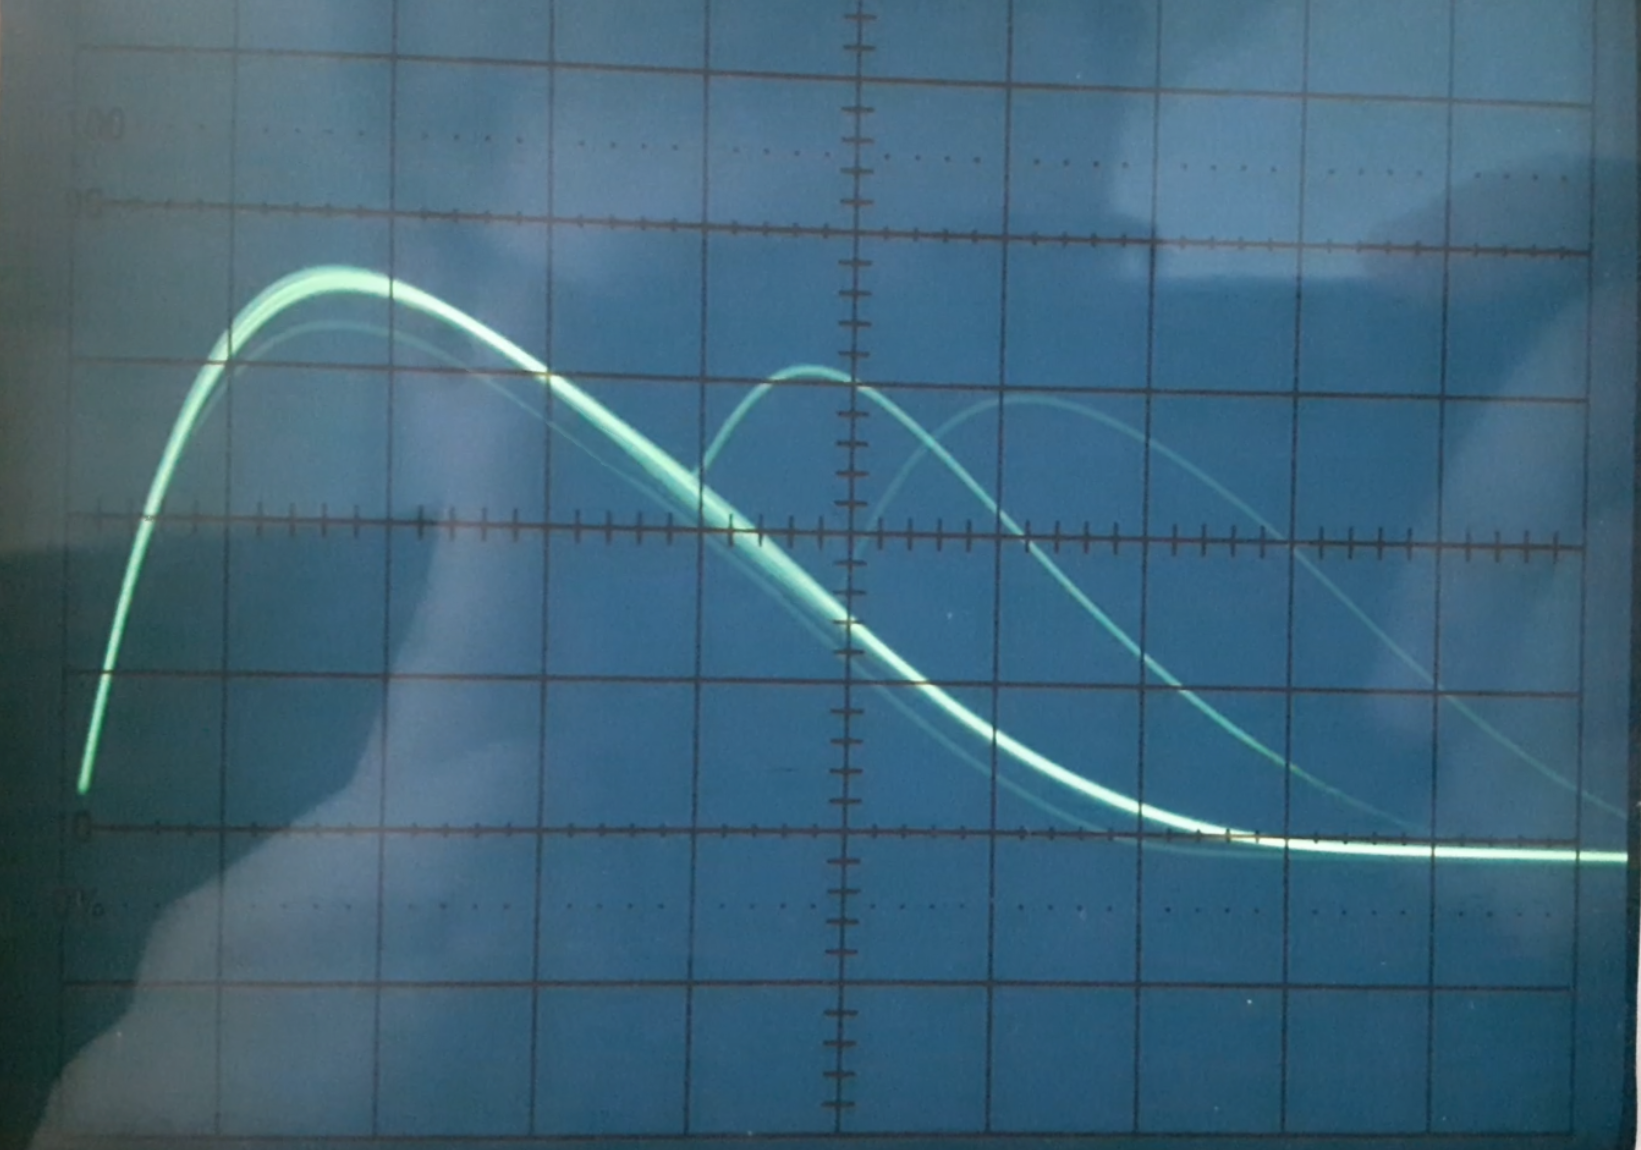
\includegraphics[width=0.95\textwidth]{content/osz.png}
  \caption{Momentaufnahme des Oszilloskopes zur Bestimmung der Totzeit der Geiger-Müller-Zählrohres.}
  \label{fig:osz}
\end{figure}

\begin{figure}
  \centering
  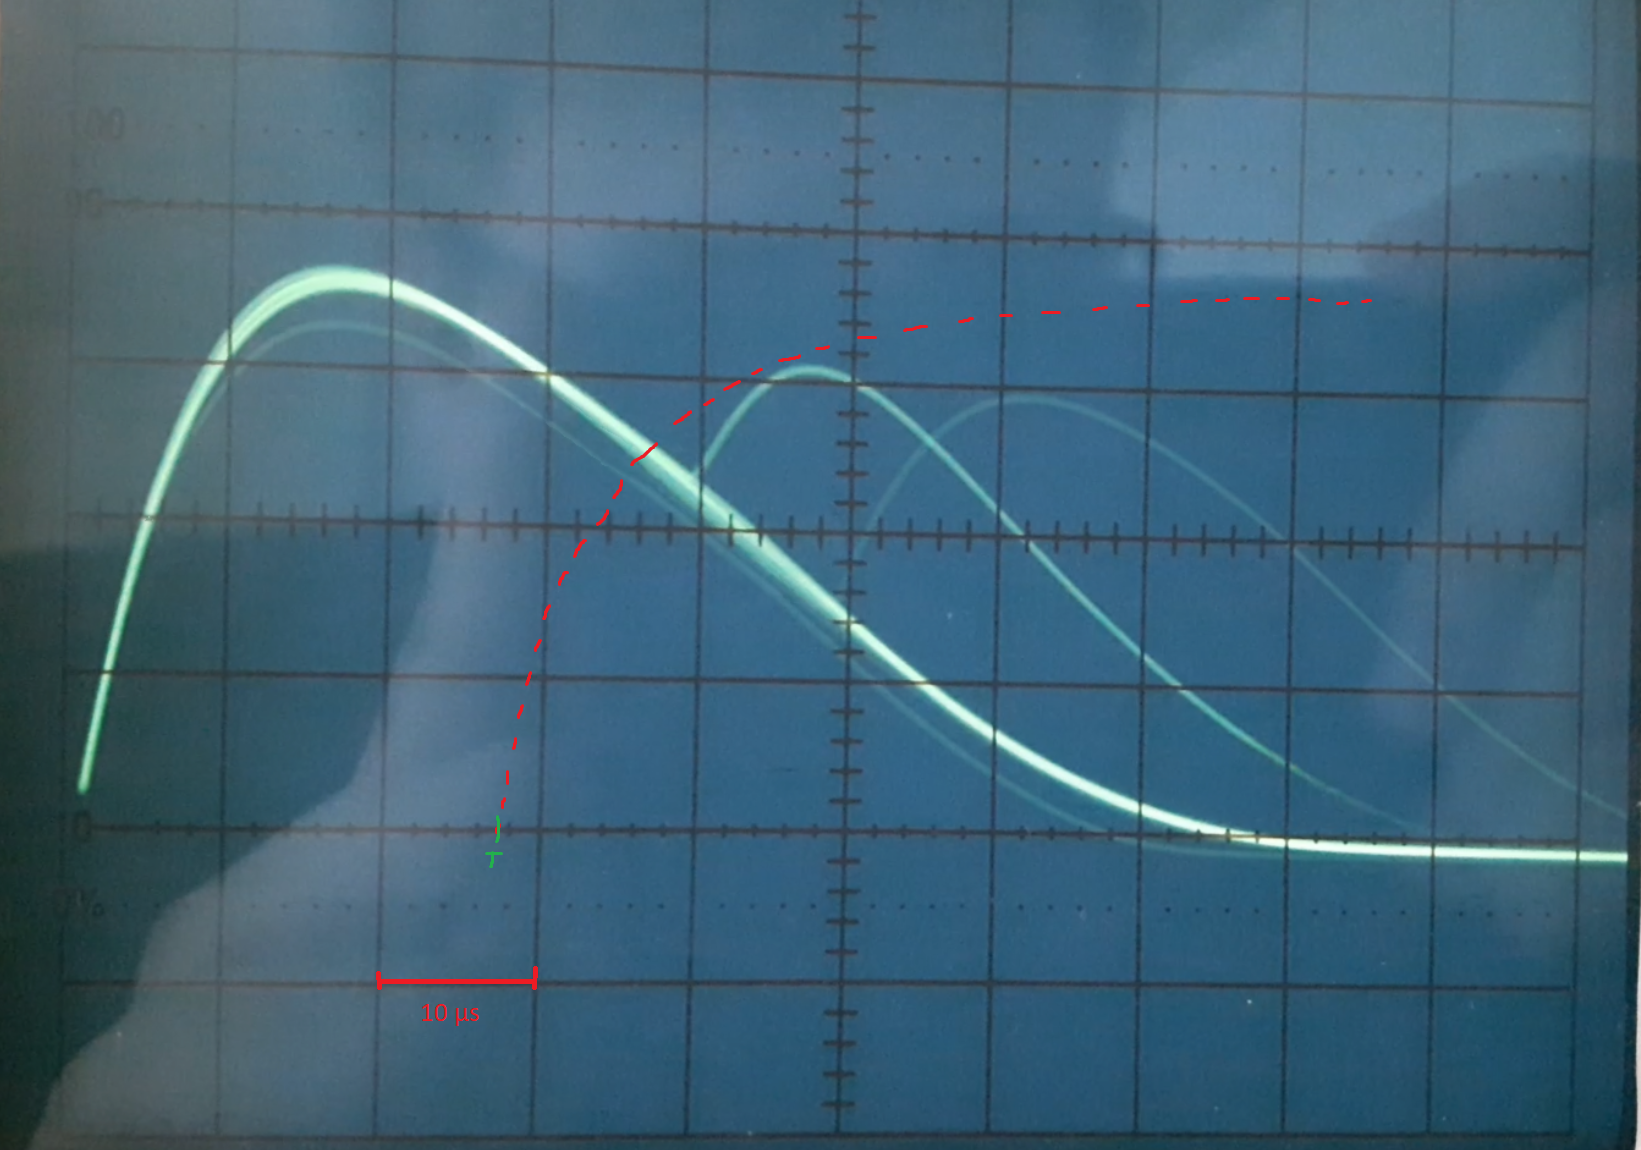
\includegraphics[width=0.95\textwidth]{content/osz_m_skizze.png}
  \caption{Momentaufnahme mit eingezeichneter Skizze des Oszilloskopes zur Bestimmung der Totzeit der Geiger-Müller-Zählrohres.}
  \label{fig:osz-m-skizze}
\end{figure}

Des Weiteren wird die Totzeit mittels des Oszilloskopes bestimmt. In \autoref{fig:osz} ist die Momentaufnahme zu sehen, bei der der Nebenpeak am weitesten links zu bemerken ist.
Durch Fortsetzung der Linien, wie in \autoref{fig:tot} zu sehen, wird die Totzeit zu

\begin{center}
    $T_\text{Osz} = (30 \pm 10)$ µs
\end{center}

bestimmt.

Über die Stromstärken in \autoref{tab:charak} lassen sich nach 

\begin{equation}
    \Delta Q = I \cdot \frac{\Delta t}{Z}
\end{equation}

die Ladungen pro Ion berechnen, 
wobei das Zeitintervall $\Delta t = 150 \, \symup{s}$ beträgt.
Die entsprechend entstehenden Werte sind in \autoref{tab:ladung} zu finden.
Dabei berechnen sich die jeweiligen Fehler nach Gauß über

\begin{equation}
    \Delta (\Delta Q) = \bigg( \frac{I_i \cdot t}{Z_i^2} \bigg) \cdot \Delta Z_i.
\end{equation}

\begin{table}[!htp]
\centering
\caption{Gemessene Stromstärken zu bestimmenten Spannungen und daraus berechnete freigesetzte Ladungsmengen.}
\label{tab:ladung}
\begin{tabular}{S[table-format=3.0] S[table-format=1.1] S[table-format=5.0] @{${}\pm{}$} S[table-format=3.0] S[table-format=1.2] @{${}\pm{}$} S[table-format=1.2] S[table-format=1.2] @{${}\pm{}$} S[table-format=1.2]}
\toprule
{$U$ / V} & {$I$ / µA} & \multicolumn{2}{c}{$Z$} & \multicolumn{2}{c}{$Q$ / nC} & \multicolumn{2}{c}{$Q$ / $10^{10} \cdot e_0$} \\
\midrule
380 & 0.2 & 11045 & 105 & 2.72 & 0.03 & 1.70 & 0.02 \\
520 & 0.4 & 11174 & 106 & 5.37 & 0.05 & 3.35 & 0.03 \\
680 & 0.6 & 11444 & 107 & 7.86 & 0.07 & 4.91 & 0.05 \\
\bottomrule
\end{tabular}
\end{table}